\documentclass[]{article}
\usepackage{lmodern}
\usepackage{amssymb,amsmath}
\usepackage{ifxetex,ifluatex}
\usepackage{fixltx2e} % provides \textsubscript
\ifnum 0\ifxetex 1\fi\ifluatex 1\fi=0 % if pdftex
  \usepackage[T1]{fontenc}
  \usepackage[utf8]{inputenc}
\else % if luatex or xelatex
  \ifxetex
    \usepackage{mathspec}
  \else
    \usepackage{fontspec}
  \fi
  \defaultfontfeatures{Ligatures=TeX,Scale=MatchLowercase}
\fi
% use upquote if available, for straight quotes in verbatim environments
\IfFileExists{upquote.sty}{\usepackage{upquote}}{}
% use microtype if available
\IfFileExists{microtype.sty}{%
\usepackage{microtype}
\UseMicrotypeSet[protrusion]{basicmath} % disable protrusion for tt fonts
}{}
\usepackage[margin=1in]{geometry}
\usepackage{hyperref}
\hypersetup{unicode=true,
            pdftitle={Spatial R course - 3},
            pdfauthor={Tobias Andermann},
            pdfborder={0 0 0},
            breaklinks=true}
\urlstyle{same}  % don't use monospace font for urls
\usepackage{color}
\usepackage{fancyvrb}
\newcommand{\VerbBar}{|}
\newcommand{\VERB}{\Verb[commandchars=\\\{\}]}
\DefineVerbatimEnvironment{Highlighting}{Verbatim}{commandchars=\\\{\}}
% Add ',fontsize=\small' for more characters per line
\usepackage{framed}
\definecolor{shadecolor}{RGB}{248,248,248}
\newenvironment{Shaded}{\begin{snugshade}}{\end{snugshade}}
\newcommand{\AlertTok}[1]{\textcolor[rgb]{0.94,0.16,0.16}{#1}}
\newcommand{\AnnotationTok}[1]{\textcolor[rgb]{0.56,0.35,0.01}{\textbf{\textit{#1}}}}
\newcommand{\AttributeTok}[1]{\textcolor[rgb]{0.77,0.63,0.00}{#1}}
\newcommand{\BaseNTok}[1]{\textcolor[rgb]{0.00,0.00,0.81}{#1}}
\newcommand{\BuiltInTok}[1]{#1}
\newcommand{\CharTok}[1]{\textcolor[rgb]{0.31,0.60,0.02}{#1}}
\newcommand{\CommentTok}[1]{\textcolor[rgb]{0.56,0.35,0.01}{\textit{#1}}}
\newcommand{\CommentVarTok}[1]{\textcolor[rgb]{0.56,0.35,0.01}{\textbf{\textit{#1}}}}
\newcommand{\ConstantTok}[1]{\textcolor[rgb]{0.00,0.00,0.00}{#1}}
\newcommand{\ControlFlowTok}[1]{\textcolor[rgb]{0.13,0.29,0.53}{\textbf{#1}}}
\newcommand{\DataTypeTok}[1]{\textcolor[rgb]{0.13,0.29,0.53}{#1}}
\newcommand{\DecValTok}[1]{\textcolor[rgb]{0.00,0.00,0.81}{#1}}
\newcommand{\DocumentationTok}[1]{\textcolor[rgb]{0.56,0.35,0.01}{\textbf{\textit{#1}}}}
\newcommand{\ErrorTok}[1]{\textcolor[rgb]{0.64,0.00,0.00}{\textbf{#1}}}
\newcommand{\ExtensionTok}[1]{#1}
\newcommand{\FloatTok}[1]{\textcolor[rgb]{0.00,0.00,0.81}{#1}}
\newcommand{\FunctionTok}[1]{\textcolor[rgb]{0.00,0.00,0.00}{#1}}
\newcommand{\ImportTok}[1]{#1}
\newcommand{\InformationTok}[1]{\textcolor[rgb]{0.56,0.35,0.01}{\textbf{\textit{#1}}}}
\newcommand{\KeywordTok}[1]{\textcolor[rgb]{0.13,0.29,0.53}{\textbf{#1}}}
\newcommand{\NormalTok}[1]{#1}
\newcommand{\OperatorTok}[1]{\textcolor[rgb]{0.81,0.36,0.00}{\textbf{#1}}}
\newcommand{\OtherTok}[1]{\textcolor[rgb]{0.56,0.35,0.01}{#1}}
\newcommand{\PreprocessorTok}[1]{\textcolor[rgb]{0.56,0.35,0.01}{\textit{#1}}}
\newcommand{\RegionMarkerTok}[1]{#1}
\newcommand{\SpecialCharTok}[1]{\textcolor[rgb]{0.00,0.00,0.00}{#1}}
\newcommand{\SpecialStringTok}[1]{\textcolor[rgb]{0.31,0.60,0.02}{#1}}
\newcommand{\StringTok}[1]{\textcolor[rgb]{0.31,0.60,0.02}{#1}}
\newcommand{\VariableTok}[1]{\textcolor[rgb]{0.00,0.00,0.00}{#1}}
\newcommand{\VerbatimStringTok}[1]{\textcolor[rgb]{0.31,0.60,0.02}{#1}}
\newcommand{\WarningTok}[1]{\textcolor[rgb]{0.56,0.35,0.01}{\textbf{\textit{#1}}}}
\usepackage{graphicx,grffile}
\makeatletter
\def\maxwidth{\ifdim\Gin@nat@width>\linewidth\linewidth\else\Gin@nat@width\fi}
\def\maxheight{\ifdim\Gin@nat@height>\textheight\textheight\else\Gin@nat@height\fi}
\makeatother
% Scale images if necessary, so that they will not overflow the page
% margins by default, and it is still possible to overwrite the defaults
% using explicit options in \includegraphics[width, height, ...]{}
\setkeys{Gin}{width=\maxwidth,height=\maxheight,keepaspectratio}
\IfFileExists{parskip.sty}{%
\usepackage{parskip}
}{% else
\setlength{\parindent}{0pt}
\setlength{\parskip}{6pt plus 2pt minus 1pt}
}
\setlength{\emergencystretch}{3em}  % prevent overfull lines
\providecommand{\tightlist}{%
  \setlength{\itemsep}{0pt}\setlength{\parskip}{0pt}}
\setcounter{secnumdepth}{0}
% Redefines (sub)paragraphs to behave more like sections
\ifx\paragraph\undefined\else
\let\oldparagraph\paragraph
\renewcommand{\paragraph}[1]{\oldparagraph{#1}\mbox{}}
\fi
\ifx\subparagraph\undefined\else
\let\oldsubparagraph\subparagraph
\renewcommand{\subparagraph}[1]{\oldsubparagraph{#1}\mbox{}}
\fi

%%% Use protect on footnotes to avoid problems with footnotes in titles
\let\rmarkdownfootnote\footnote%
\def\footnote{\protect\rmarkdownfootnote}

%%% Change title format to be more compact
\usepackage{titling}

% Create subtitle command for use in maketitle
\providecommand{\subtitle}[1]{
  \posttitle{
    \begin{center}\large#1\end{center}
    }
}

\setlength{\droptitle}{-2em}

  \title{Spatial R course - 3}
    \pretitle{\vspace{\droptitle}\centering\huge}
  \posttitle{\par}
    \author{Tobias Andermann}
    \preauthor{\centering\large\emph}
  \postauthor{\par}
      \predate{\centering\large\emph}
  \postdate{\par}
    \date{5/25/2020}


\begin{document}
\maketitle

\hypertarget{accessing-biodiveristy-data-through-web-services-gbif}{%
\subsection{Accessing biodiveristy data through web services
(GBIF)}\label{accessing-biodiveristy-data-through-web-services-gbif}}

In this tutorial we will go through some different functions related to
downloading biodiveristy data, mostly from GBIF. The point of this
tutorial is to provide you the tools to properly download such data in
publication quality (DOI-assigned and thus tracable) and to provide you
with some handy plotting functions to display the downloaded data.

Dependencies:

\begin{Shaded}
\begin{Highlighting}[]
\KeywordTok{library}\NormalTok{(sp)}
\KeywordTok{library}\NormalTok{(raster)}
\KeywordTok{library}\NormalTok{(sf)}
\KeywordTok{library}\NormalTok{(rgbif)}
\KeywordTok{library}\NormalTok{(ggplot2)}
\end{Highlighting}
\end{Shaded}

\hypertarget{define-taxonomy}{%
\subsubsection{1. Define taxonomy}\label{define-taxonomy}}

Taxonomy can be a tricky topic. Several different names exist for many
taxa, variations being caused by misspellings, different synonyms and
regional differences in common names for species. If you want to extract
all records for a certain taxon, you first needs to define a coherent
taxonomy and in the worst case you need to sync all available datasets
to this chosen taxonomy. This can be a rabbit-hole that can make the
collection of large datasets from public databases very time consuming.
Luckily GBIF is working with one consistent taxonomy, which most records
are assigned to. In this tutorial we will work with this GBIF backbone
taxonomy (NUB). Check out the description of the GBIF taxonomy under
\href{https://www.gbif.org/dataset/d7dddbf4-2cf0-4f39-9b2a-bb099caae36c\#description}{this
link} to understand how this taxonomy is derived and how to cite it.

The following identifier points to the NUB taxonomy, which will make
more sense in a little bit.

\begin{Shaded}
\begin{Highlighting}[]
\NormalTok{nub <-}\StringTok{ 'd7dddbf4-2cf0-4f39-9b2a-bb099caae36c'}
\end{Highlighting}
\end{Shaded}

\hypertarget{pick-a-speciesgenusfamily}{%
\subsubsection{2. Pick a
species/genus/family}\label{pick-a-speciesgenusfamily}}

Pick your own species, genus, or family of interest, for which you want
to extract occurrence data from GBIF. If you are feeling sufficiently
familiar with R, go ahead and extract occurrence data for multiple taxa,
which at the end will yield the most interesting results when plotting
the data. In this tutorial we will use an example species but it's
strongly encouraged for you to go through the exercise with your own
picked taxon (doens't have to be a species, can be a smaller or larger
taxonomic entity).

\begin{Shaded}
\begin{Highlighting}[]
\NormalTok{taxon_name <-}\StringTok{ "Turdus merula"}
\end{Highlighting}
\end{Shaded}

There is a useful search function in rgbif called
\texttt{name\_suggest()}. This will return any matches with your
provided taxon name and return the name as well as the taxonomic rank of
the match:

\begin{Shaded}
\begin{Highlighting}[]
\KeywordTok{library}\NormalTok{(rgbif)}
\KeywordTok{name_suggest}\NormalTok{(}\DataTypeTok{q=}\NormalTok{taxon_name)}
\end{Highlighting}
\end{Shaded}

\begin{verbatim}
## # A tibble: 13 x 3
##        key canonicalName              rank      
##      <int> <chr>                      <chr>     
##  1 2490719 Turdus merula              SPECIES   
##  2 6094911 Turdus merula sowerbyi     SUBSPECIES
##  3 9173280 Turdus merula nigropileus  SUBSPECIES
##  4 6094902 Turdus merula mandarinus   SUBSPECIES
##  5 6094954 Turdus merula cabrerae     SUBSPECIES
##  6 8917151 Turdus merula mallorcae    SUBSPECIES
##  7 9095250 Turdus merula buddae       SUBSPECIES
##  8 6094935 Turdus merula syriacus     SUBSPECIES
##  9 6094947 Turdus merula mauritanicus SUBSPECIES
## 10 5846244 Turdus merula intermedius  SUBSPECIES
## 11 6094940 Turdus merula aterrimus    SUBSPECIES
## 12 6171845 Turdus merula merula       SUBSPECIES
## 13 6094960 Turdus merula azorensis    SUBSPECIES
\end{verbatim}

\hypertarget{check-taxonomic-information}{%
\subsubsection{3. Check taxonomic
information}\label{check-taxonomic-information}}

Now we use the \texttt{name\_lookup()} function of the rgbif package to
check if our picked taxon exists in the chosen GBIF backbone taxonomy
and what information is stored with it. In order for the function to
find our taxon in the taxonomy, we need to provide the rank that the
taxon name represents (is it a subspecies, species, genus, or family
name?). We can extract the correct rank classification from the results
of the \texttt{name\_suggest()} function as shown above. In this example
we're working with a taxon name that is on the species level. Accepted
ranks are:
\texttt{CLASS,\ CULTIVAR,\ CULTIVAR\_GROUP,\ DOMAIN,\ FAMILY,\ FORM,\ GENUS,\ INFORMAL,\ INFRAGENERIC\_NAME,\ INFRAORDER,\ INFRASPECIFIC\_NAME,\ INFRASUBSPECIFIC\_NAME,\ KINGDOM,\ ORDER,\ PHYLUM,\ SECTION,\ SERIES,\ SPECIES,\ STRAIN,\ SUBCLASS,\ SUBFAMILY,\ SUBFORM,\ SUBGENUS,\ SUBKINGDOM,\ SUBORDER,\ SUBPHYLUM,\ SUBSECTION,\ SUBSERIES,\ SUBSPECIES,\ SUBTRIBE,\ SUBVARIETY,\ SUPERCLASS,\ SUPERFAMILY,\ SUPERORDER,\ SUPERPHYLUM,\ SUPRAGENERIC\_NAME,\ TRIBE,\ UNRANKED,\ VARIETY}
If you are uncertain about how to parse your taxon name into this
function, check the helpfunction by executing \texttt{?name\_lookup()}
in R. Note that in the command below we are using the
\texttt{datasetKey=nub} settings, which is the GBIF standard taxonomy we
defined earlier.

\begin{Shaded}
\begin{Highlighting}[]
\NormalTok{rank =}\StringTok{ 'species'}
\NormalTok{taxon_taxonomy_data =}\StringTok{ }\KeywordTok{name_lookup}\NormalTok{(}\DataTypeTok{query=}\NormalTok{taxon_name, }\DataTypeTok{rank=}\NormalTok{rank, }\DataTypeTok{datasetKey=}\NormalTok{nub, }\DataTypeTok{limit=}\DecValTok{1}\NormalTok{)}
\NormalTok{taxon_taxonomy_data}
\end{Highlighting}
\end{Shaded}

\begin{verbatim}
## $meta
## # A tibble: 1 x 4
##   offset limit endOfRecords count
##    <int> <int> <lgl>        <int>
## 1      0     1 FALSE           15
## 
## $data
## # A tibble: 1 x 34
##      key scientificName datasetKey constituentKey parentKey parent kingdom
##    <int> <chr>          <chr>      <chr>              <int> <chr>  <chr>  
## 1 2.49e6 Turdus merula~ d7dddbf4-~ 7ddf754f-d193~   2490714 Turdus Animal~
## # ... with 27 more variables: phylum <chr>, order <chr>, family <chr>,
## #   genus <chr>, species <chr>, kingdomKey <int>, phylumKey <int>,
## #   classKey <int>, orderKey <int>, familyKey <int>, genusKey <int>,
## #   speciesKey <int>, canonicalName <chr>, authorship <chr>,
## #   publishedIn <chr>, nameType <chr>, taxonomicStatus <chr>, rank <chr>,
## #   origin <chr>, numDescendants <int>, numOccurrences <int>,
## #   extinct <lgl>, habitats <chr>, nomenclaturalStatus <lgl>,
## #   threatStatuses <chr>, synonym <lgl>, class <chr>
## 
## $facets
## NULL
## 
## $hierarchies
## $hierarchies$`2490719`
##   rankkey          name
## 1       1      Animalia
## 2      44      Chordata
## 3     212          Aves
## 4     729 Passeriformes
## 5    5290      Turdidae
## 6 2490714        Turdus
## 
## 
## $names
## $names$`2490719`
##                           vernacularName language
## 1                                  Amsel      deu
## 2                              blackbird      eng
## 3                                  merel      nld
## 4                             merle noir      fra
## 5                              blackbird      eng
## 6                     Eurasian Blackbird      eng
## 7                             Merle noir      fra
## 8                       Common Blackbird      eng
## 9                     Eurasian Blackbird      eng
## 10 Eurasian Blackbird / Common Blackbird      eng
## 11                      Common Blackbird      eng
## 12                    Eurasian Blackbird      eng
## 13                            Merle noir      fra
## 14                      common blackbird      eng
## 15                                 Amsel      deu
## 16                      common blackbird      eng
## 17                             karatavuk      tur
## 18                                 merel      nld
## 19                            merle noir      fra
## 20                               mulleja      sqi
## 21                               mullija      sqi
## 22                             mullizeza      sqi
## 23                             mwyalchen      cym
## 24                              mëllënja      sqi
## 25                        qofka e murrme      sqi
## 26                                 qukla      sqi
## 27                            svarttrost      nor
## 28                       Κοινός Κότσυφας      ell
## 29                                   Кос      bul
## 30                                 Amsel         
## 31                    Eurasian blackbird         
## 32                             blackbird         
## 33                                 Amsel      deu
## 34                             Blackbird      eng
## 35                           Mirlo Común      spa
## 36                           Mustarastas      fin
## 37                            Merle noir      fra
## 38                           Fekete rigó      hun
## 39                                 Merlo      ita
## 40                                 Merel      nld
## 41                                   Kos      pol
## 42                           Melro-preto      por
## 43                              Koltrast      swe
## 44                               Solsort      dan
## 45                                 Amsel      deu
## 46                      Common Blackbird      eng
## 47                           Kvørkveggja      fao
## 48                           Mustarastas      fin
## 49                               Solsort      dan
## 50                            Svarttrost      nob
## 51                          Svartßröstur      isl
## 52                              koltrast      swe
## 53                                 Merel      nld
## 54                        Zwarte lijster      nld
## 55                      Common Blackbird      eng
## 56                    Eurasian Blackbird      eng
## 57                            merle noir      fra
## 58                                 Amsel      deu
## 59                      Common Blackbird      eng
## 60                    Eurasian Blackbird      eng
## 61                            merle noir      fra
## 62                                 Amsel      deu
## 63                      Common Blackbird      eng
## 64                                 Merel      nld
## 65                            Merle noir      fra
## 66                                 Merlo      ita
## 67                           Mirlo Común      spa
## 68                               Solsort      dan
## 69                            Svarttrost      nor
## 70                          drozd čierny      slk
## 71                           fekete rigó      hun
## 72                     juodasis strazdas      lit
## 73                              koltrast      swe
## 74                                   kos      slv
## 75                       kos (zwyczajny)      pol
## 76                             kos černý      ces
## 77                   melnais mežastrazds      lav
## 78                                 melro      por
## 79                                 merla      cat
## 80                           mustarastas      fin
## 81                            musträstas      est
## 82                          Чёрный дрозд      rus
## 83                                  乌鸫      zho
## 84                                  烏鶇      zho
\end{verbatim}

You can see there is a lot of useful data stored in this taxonomy. First
we can extract the \textbf{numerical taxon id} which we will use in
following steps to extract occurrence records for this taxon. The
advatange of using a numerical id is that the taxon is unmistakenly
defined and will not anymore be subject to misspellings and different
synonyms from here on.

\begin{Shaded}
\begin{Highlighting}[]
\NormalTok{taxon_id =}\StringTok{ }\NormalTok{taxon_taxonomy_data}\OperatorTok{$}\NormalTok{data}\OperatorTok{$}\NormalTok{key}
\NormalTok{taxon_id}
\end{Highlighting}
\end{Shaded}

\begin{verbatim}
## [1] 2490719
\end{verbatim}

The \texttt{name\_lookup()} function also provides us the taxon ids of
the encompassing taxa higher up in the taxonomic hierarchy. In this
example it tells us that the blackbird belongs to the genus Turdus in
the family Turdidae etc.

\begin{Shaded}
\begin{Highlighting}[]
\NormalTok{taxon_taxonomy_data}\OperatorTok{$}\NormalTok{hierarchies}
\end{Highlighting}
\end{Shaded}

\begin{verbatim}
## $`2490719`
##   rankkey          name
## 1       1      Animalia
## 2      44      Chordata
## 3     212          Aves
## 4     729 Passeriformes
## 5    5290      Turdidae
## 6 2490714        Turdus
\end{verbatim}

From the output we can extract the ID of the encompassing genus, which
we will be using later on in the tutorial, since we will to work with
data of several species. If your genus only has a single species, maybe
pick a different genus.

\begin{Shaded}
\begin{Highlighting}[]
\NormalTok{genus_ID =}\StringTok{ }\NormalTok{taxon_taxonomy_data}\OperatorTok{$}\NormalTok{data}\OperatorTok{$}\NormalTok{genusKey}
\NormalTok{genus_ID}
\end{Highlighting}
\end{Shaded}

\begin{verbatim}
## [1] 2490714
\end{verbatim}

Alternatively you can also extract the ID of the parent taxon in
general, e.g.~if you looked up data for a genus you can extract the
family ID like this (in the case of my example here it is the ID of the
genus since I looked up the taxonomy of a species, which I stored as
\texttt{taxon\_taxonomy\_data}):

\begin{Shaded}
\begin{Highlighting}[]
\NormalTok{genus_ID =}\StringTok{ }\NormalTok{taxon_taxonomy_data}\OperatorTok{$}\NormalTok{data}\OperatorTok{$}\NormalTok{parentKey}
\NormalTok{genus_ID}
\end{Highlighting}
\end{Shaded}

\begin{verbatim}
## [1] 2490714
\end{verbatim}

We can also retrieve a list of popular names (vernacular names) in
different languages for our taxon. This list might come in handy if we
are to combine the GBIF occurrence data with data from other
data-sources, which may not have adopted the same taxonomy. In that case
we could search for any matches with this list of vernacular names.

\begin{Shaded}
\begin{Highlighting}[]
\NormalTok{taxon_taxonomy_data}\OperatorTok{$}\NormalTok{names[[}\DecValTok{1}\NormalTok{]]}\OperatorTok{$}\NormalTok{vernacularName}
\end{Highlighting}
\end{Shaded}

\begin{verbatim}
##  [1] Amsel                                
##  [2] blackbird                            
##  [3] merel                                
##  [4] merle noir                           
##  [5] blackbird                            
##  [6] Eurasian Blackbird                   
##  [7] Merle noir                           
##  [8] Common Blackbird                     
##  [9] Eurasian Blackbird                   
## [10] Eurasian Blackbird / Common Blackbird
## [11] Common Blackbird                     
## [12] Eurasian Blackbird                   
## [13] Merle noir                           
## [14] common blackbird                     
## [15] Amsel                                
## [16] common blackbird                     
## [17] karatavuk                            
## [18] merel                                
## [19] merle noir                           
## [20] mulleja                              
## [21] mullija                              
## [22] mullizeza                            
## [23] mwyalchen                            
## [24] mëllënja                             
## [25] qofka e murrme                       
## [26] qukla                                
## [27] svarttrost                           
## [28] Κοινός Κότσυφας                      
## [29] Кос                                  
## [30] Amsel                                
## [31] Eurasian blackbird                   
## [32] blackbird                            
## [33] Amsel                                
## [34] Blackbird                            
## [35] Mirlo Común                          
## [36] Mustarastas                          
## [37] Merle noir                           
## [38] Fekete rigó                          
## [39] Merlo                                
## [40] Merel                                
## [41] Kos                                  
## [42] Melro-preto                          
## [43] Koltrast                             
## [44] Solsort                              
## [45] Amsel                                
## [46] Common Blackbird                     
## [47] Kvørkveggja                          
## [48] Mustarastas                          
## [49] Solsort                              
## [50] Svarttrost                           
## [51] Svartßröstur                         
## [52] koltrast                             
## [53] Merel                                
## [54] Zwarte lijster                       
## [55] Common Blackbird                     
## [56] Eurasian Blackbird                   
## [57] merle noir                           
## [58] Amsel                                
## [59] Common Blackbird                     
## [60] Eurasian Blackbird                   
## [61] merle noir                           
## [62] Amsel                                
## [63] Common Blackbird                     
## [64] Merel                                
## [65] Merle noir                           
## [66] Merlo                                
## [67] Mirlo Común                          
## [68] Solsort                              
## [69] Svarttrost                           
## [70] drozd čierny                         
## [71] fekete rigó                          
## [72] juodasis strazdas                    
## [73] koltrast                             
## [74] kos                                  
## [75] kos (zwyczajny)                      
## [76] kos černý                            
## [77] melnais mežastrazds                  
## [78] melro                                
## [79] merla                                
## [80] mustarastas                          
## [81] musträstas                           
## [82] Чёрный дрозд                         
## [83] 乌鸫                                 
## [84] 烏鶇                                 
## 50 Levels: Amsel blackbird merel merle noir ... 烏鶇
\end{verbatim}

\hypertarget{download-occurrence-data}{%
\subsubsection{4. Download occurrence
data}\label{download-occurrence-data}}

Now we have determined our taxon ID and can proceed downloading
occurrence data. Downloading occurrence data from GBIF can be done using
the \texttt{occ\_search()} function of the rgbif package. We already
touched upon this in yesterday's tutorial, but we'll explore the gbif
\texttt{occ\_search()} function in some more detail today.

Before we start downloading, it is usually a good idea to check first
how many occurrences will be downloaded. In general it takes quite a
while to download hundreds of thousands of records, while a few thousand
up to tens of thousands might be feasible for this exercise. In order to
get a count of matches, we only download the metadata of our search
(instead of the actual data) by setting
\texttt{return\ =\ \textquotesingle{}meta\textquotesingle{}}. We then
call the count value from the exported metadata:

\begin{Shaded}
\begin{Highlighting}[]
\KeywordTok{occ_search}\NormalTok{(}\DataTypeTok{taxonKey=}\NormalTok{taxon_id, }\DataTypeTok{hasCoordinate =} \OtherTok{TRUE}\NormalTok{, }\DataTypeTok{return =}  \StringTok{"meta"}\NormalTok{)}\OperatorTok{$}\NormalTok{count}
\end{Highlighting}
\end{Shaded}

\begin{verbatim}
## [1] 4853745
\end{verbatim}

You see in my case there are almost 5 Million records of my target
species! If you want to restrict your search by searching for a specific
locality/region/country, there are several flags that can be used to
restrict the search geographically. Some examples are:

\begin{Shaded}
\begin{Highlighting}[]
\NormalTok{locality =}\StringTok{ }\KeywordTok{c}\NormalTok{(}\StringTok{"Gothenburg"}\NormalTok{, }\StringTok{"Göteborg"}\NormalTok{)}

\NormalTok{continent =}\StringTok{ 'europe'}

\NormalTok{country =}\StringTok{ 'SE'}
\end{Highlighting}
\end{Shaded}

In my case I will proceed with donwloading all occurrences for Sweden
(country = `SE'). Feel free to select whatever region or city you're
interested in.

\begin{Shaded}
\begin{Highlighting}[]
\KeywordTok{occ_search}\NormalTok{(}\DataTypeTok{taxonKey=}\NormalTok{taxon_id, }\DataTypeTok{hasCoordinate =} \OtherTok{TRUE}\NormalTok{, }\DataTypeTok{return =}  \StringTok{"meta"}\NormalTok{,}\DataTypeTok{country =} \StringTok{'SE'}\NormalTok{)}\OperatorTok{$}\NormalTok{count}
\end{Highlighting}
\end{Shaded}

\begin{verbatim}
## [1] 748102
\end{verbatim}

If your count of datapoints is higher than 20,000 you probably want to
set a limit to the number of occurrences to be downloaded for the
purpose of this exercise, since it will otherwise take a very long time.
You can set a download limit in the \texttt{occ\_search()} function,
using the limit=NUM flag, where NUM is the number of records you want to
export. In this case I'm setting this number to 5,000. Downloading this
many records may take a minute. If your taxon of choice doesn't have
that many records, it will donwload as many records as there are and it
might thus be finished a lot faster.

\begin{Shaded}
\begin{Highlighting}[]
\NormalTok{records <-}\StringTok{ }\KeywordTok{occ_search}\NormalTok{(}\DataTypeTok{taxonKey=}\NormalTok{taxon_id, }\DataTypeTok{return=}\StringTok{"data"}\NormalTok{, }\DataTypeTok{hasCoordinate=}\OtherTok{TRUE}\NormalTok{, }\DataTypeTok{limit=}\DecValTok{5000}\NormalTok{,}\DataTypeTok{country =} \StringTok{'SE'}\NormalTok{)}
\end{Highlighting}
\end{Shaded}

As a little side note, if you want to download occurrence data for a
list of species names (\texttt{spp\_names}) you can do it like this, by
first getting the taxon ids (\texttt{keys}) for all your target species,
and then feddign this list of ids into the \texttt{occ\_search()}
function. This will return a list of output dataframes, one for each
species.

\begin{Shaded}
\begin{Highlighting}[]
\NormalTok{spp_names <-}\StringTok{ }\KeywordTok{c}\NormalTok{(}\StringTok{'Hepatica nobilis'}\NormalTok{, }\StringTok{'Anemone nemorosa'}\NormalTok{, }\StringTok{'Taraxacum officinale'}\NormalTok{, }\StringTok{'Trifolium pratense'}\NormalTok{)  }
\NormalTok{keys <-}\StringTok{ }\KeywordTok{sapply}\NormalTok{(spp_names, }\ControlFlowTok{function}\NormalTok{(x) }\KeywordTok{name_backbone}\NormalTok{(}\DataTypeTok{name=}\NormalTok{x, }\DataTypeTok{kingdom=}\StringTok{'plants'}\NormalTok{)}\OperatorTok{$}\NormalTok{speciesKey, }\DataTypeTok{USE.NAMES=}\OtherTok{FALSE}\NormalTok{)}
\NormalTok{spp <-}\StringTok{ }\KeywordTok{occ_search}\NormalTok{(}\DataTypeTok{taxonKey=}\NormalTok{keys, }\DataTypeTok{limit=}\DecValTok{100}\NormalTok{, }\DataTypeTok{return=}\StringTok{'data'}\NormalTok{, }\DataTypeTok{country=}\StringTok{'NO'}\NormalTok{, }\DataTypeTok{hasCoordinate=}\OtherTok{TRUE}\NormalTok{) }\CommentTok{## return list}
\end{Highlighting}
\end{Shaded}

\hypertarget{plot-the-occurrence-data}{%
\subsubsection{5. Plot the occurrence
data}\label{plot-the-occurrence-data}}

There is a cool plotting library
\href{https://ggplot2.tidyverse.org/}{ggplot2} which allows very easy
plotting from dataframes like the one produced from the gbif
\texttt{occ\_search()}command. ggplot2 offers tons of fancy plotting
options and is a whole science for itself. If you enjoy making nice
plots it's worth \href{(https://ggplot2.tidyverse.org/)}{checking it out
in more detail}. For now we just load the map object and we'll then use
it in the plotting command later on.

ggplot2 also has integrated commands to load map data. Using the
borders() function, we can very easily load a world map with the
following command. This stores the polygon information in a ggplot
specific format, which is different to the SpatialPolygons format of the
world polygons we were loading yesterday. You can set the color of the
map and of the filling of landmasses in this command.

\begin{Shaded}
\begin{Highlighting}[]
\KeywordTok{library}\NormalTok{(ggplot2)}
\NormalTok{map_world <-}\StringTok{ }\KeywordTok{borders}\NormalTok{(}\DataTypeTok{database =} \StringTok{"world"}\NormalTok{, }\DataTypeTok{colour =} \StringTok{"gray50"}\NormalTok{, }\DataTypeTok{fill =} \StringTok{"#383838"}\NormalTok{)}
\end{Highlighting}
\end{Shaded}

It is usually a good idea to crop the world map to the area where our
points are occurring. So let's first define the bounding box, which we
can then use to restrict the plotting to only our selected area:

\begin{Shaded}
\begin{Highlighting}[]
\NormalTok{xmin<-}\KeywordTok{min}\NormalTok{(records}\OperatorTok{$}\NormalTok{decimalLongitude)}
\NormalTok{xmax<-}\KeywordTok{max}\NormalTok{(records}\OperatorTok{$}\NormalTok{decimalLongitude)}
\NormalTok{ymin<-}\KeywordTok{min}\NormalTok{(records}\OperatorTok{$}\NormalTok{decimalLatitude)}
\NormalTok{ymax<-}\KeywordTok{max}\NormalTok{(records}\OperatorTok{$}\NormalTok{decimalLatitude)}
\end{Highlighting}
\end{Shaded}

Now let's plot our points on the map, colored by species name. The logic
of the ggplot syntax is accumulative. That means you can add additonal
layers/settings to the command by adding lines connnected with a
\texttt{+} sign.

First we just call the function \texttt{ggplot()}, then tell it to plot
our \texttt{map\_world} object we created above, then add our gbid
dataframe (\texttt{records}) using the \texttt{geom\_point()} function.
Within the \texttt{geom\_point()} commadn we use \texttt{aes()} where we
provide the column names in the dataframe that correspond to the
x-coordinates (\texttt{x=}), y-coordinates (\texttt{y=}), and the name
of the column we want to color our points by (\texttt{colour=}), which
in this case is by the species column. Then crop the map around the
borders (xmin,xmax,ymin,ymax) defined in the previous step (based on the
spread of the data), and finally we add a legend using the
\texttt{theme()} command.

\begin{Shaded}
\begin{Highlighting}[]
\KeywordTok{ggplot}\NormalTok{() }\OperatorTok{+}
\NormalTok{map_world }\OperatorTok{+}
\KeywordTok{geom_point}\NormalTok{(}\DataTypeTok{data =}\NormalTok{ records,  }\CommentTok{# Specify the data for geom_point()}
             \KeywordTok{aes}\NormalTok{(}\DataTypeTok{x =}\NormalTok{ decimalLongitude,  }\CommentTok{# Specify the x axis as longitude}
                 \DataTypeTok{y =}\NormalTok{ decimalLatitude,}
                 \DataTypeTok{colour =}\NormalTok{ species),  }\CommentTok{# Colour the points based on species name}
             \DataTypeTok{alpha =} \FloatTok{0.4}\NormalTok{,  }\CommentTok{# Set point opacity to 40%}
             \DataTypeTok{size =} \DecValTok{1}\NormalTok{) }\OperatorTok{+}
\KeywordTok{coord_cartesian}\NormalTok{(}\DataTypeTok{xlim =} \KeywordTok{c}\NormalTok{((xmin),(xmax)), }\DataTypeTok{ylim =} \KeywordTok{c}\NormalTok{((ymin),(ymax))) }\OperatorTok{+}
\KeywordTok{theme}\NormalTok{(}\DataTypeTok{legend.position =} \StringTok{"bottom"}\NormalTok{)}
\end{Highlighting}
\end{Shaded}

\includegraphics{tutorial_3_files/figure-latex/unnamed-chunk-18-1.pdf}

You see that this is somewhat simpler than the way we did it yesterday
with loading country or world shape files from separate files and
loading them as spatial polygons, transforming the points into
SpatialPoints objects, etc. However, it is good to know and understand
how to do it the old-school way, but it's also nice to know that there
are easier and more user-freindly options out there.

The plot above looks a bit boring since it only contains the data from
my one target species. Recreate the plot for your area and target group
of choice. Make sure your dataset contains multiple species, e.g.~use
the \texttt{genus\_ID} we extracted earlier, to download and plot data
for a whole genus. Color the points by the species they belong to.

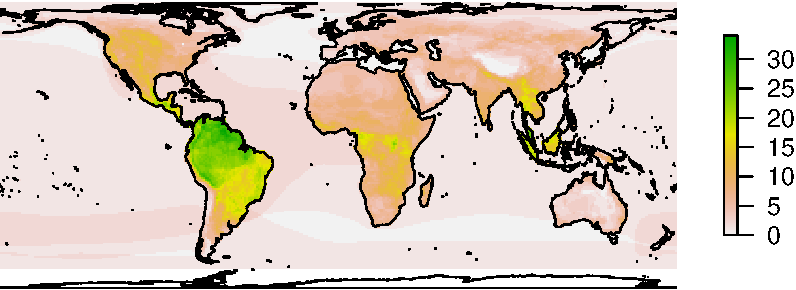
\includegraphics{tutorial_3_files/figure-latex/unnamed-chunk-19-1.pdf}

\hypertarget{citing-the-source-data}{%
\subsubsection{6. Citing the source data}\label{citing-the-source-data}}

If you want to be very thorough in your citations, you can export all
citations of the data that are present in your downloaded GBIF dataframe
(which we stored as \texttt{records}). You can easily retrieve this
information using the \texttt{gbif\_citation()} function:

\begin{Shaded}
\begin{Highlighting}[]
\KeywordTok{gbif_citation}\NormalTok{(records)}
\end{Highlighting}
\end{Shaded}

\begin{verbatim}
## [[1]]
## <<rgbif citation>>
##    Citation: Shah M, Coulson S (2020). Artportalen (Swedish Species Observation
##         System). Version 92.192. SLU Artdatabanken. Occurrence dataset
##         https://doi.org/10.15468/kllkyl accessed via GBIF.org on 2020-05-25..
##         Accessed from R via rgbif (https://github.com/ropensci/rgbif) on
##         2020-05-25
##    Rights:
\end{verbatim}

In some cases this could be a very long list of references.
Alternatively/additionally you can create your own official download
request at GBIF, which will assign a DOI to your download that can (and
should) be cited when publishing such data. The advantage is that
everybody can access the donwload and (hopefully) reproduce your
operations on the data. This is the proper way of using GBIF data for
publications.

First you need to create a user account at GBIF. This is very simple and
fast, just follow \href{https://www.gbif.org/user/profile}{this link}.
Once you created your account and activated it via email, you can
execute the lines below in R after replacing the values
\texttt{USERNAME}, \texttt{PASSWORD}, and \texttt{EMAIL} with your
account name, passwort, and email address, respectively. You only need
to do this once in this session. From here on out the rgbif package will
remember your user data, but you'll have to enter them again when you
restart R next time.

\begin{Shaded}
\begin{Highlighting}[]
\KeywordTok{options}\NormalTok{(}\DataTypeTok{gbif_user=}\StringTok{'USERNAME'}\NormalTok{)}
\KeywordTok{options}\NormalTok{(}\DataTypeTok{gbif_pwd=}\StringTok{'PASSWORD'}\NormalTok{)}
\KeywordTok{options}\NormalTok{(}\DataTypeTok{gbif_email=}\StringTok{'EMAIL'}\NormalTok{)}
\end{Highlighting}
\end{Shaded}

Now let's create a download request for all occurrences associated with
your chosen taxon. For this you can use the \texttt{occ\_download()}
command (instead of \texttt{occ\_search()} which we were using before),
where you provide the \texttt{taxonKey} and specify that you want only
records with coordinates (\texttt{hasCoordinate}). The
\texttt{type="and"} setting means that both of these requirements have
to be fulfilled (i.e.~the \texttt{taxonId} needs to match and the
records must have coordinates assigned to it).

\begin{Shaded}
\begin{Highlighting}[]
\CommentTok{# Get download key}
\NormalTok{request =}\StringTok{ }\KeywordTok{occ_download}\NormalTok{(}\KeywordTok{paste0}\NormalTok{(}\StringTok{'taxonKey ='}\NormalTok{,taxon_id),}\StringTok{'hasCoordinate = TRUE'}\NormalTok{,}\DataTypeTok{type =} \StringTok{"and"}\NormalTok{)}
\NormalTok{request}
\end{Highlighting}
\end{Shaded}

\begin{verbatim}
## <<gbif download>>
##   Username: tobiashofmann
##   E-mail: tobiashofmann@gmx.net
##   Download key: 0070605-200221144449610
\end{verbatim}

You can get more information about your download request by using the
\texttt{occ\_download\_meta()} function or by logging into your gbif
user account and checking the
\href{https://www.gbif.org/user/download}{download section}:

\begin{Shaded}
\begin{Highlighting}[]
\NormalTok{download_key =}\StringTok{ }\KeywordTok{occ_download_meta}\NormalTok{(request[}\DecValTok{1}\NormalTok{])}
\NormalTok{download_key}
\end{Highlighting}
\end{Shaded}

\begin{verbatim}
## <<gbif download metadata>>
##   Status: PREPARING
##   Format: DWCA
##   Download key: 0070605-200221144449610
##   Created: 2020-05-25T21:03:34.358+0000
##   Modified: 2020-05-25T21:03:34.358+0000
##   Download link: http://api.gbif.org/v1/occurrence/download/request/0070605-200221144449610.zip
##   Total records: 0
##   Request: 
##     type:  and
##     predicates: 
##       > type: equals, key: TAXON_KEY, value: 2490719
##       > type: equals, key: HAS_COORDINATE, value: TRUE
\end{verbatim}

It will take 10-20 minutes (depending on the number of records in your
query) for this download request to finish compiling. Once the Status:
field says \texttt{SUCCEEDED} you are ready to retrieve your data. You
can do this through R using the \texttt{occ\_download\_get()} function,
or you can instead manually download the file by clicking on download on
your GBIF webpage. When using the \texttt{occ\_download\_get()}
function, provide the path where the zipped folder should be saved
(\texttt{../output\_files/} in my case, replace with your path where you
want to save, make sure that the folder exists where you are trying to
save it).

\begin{Shaded}
\begin{Highlighting}[]
\CommentTok{#key = request[1]}
\NormalTok{key =}\StringTok{ "0006240-190415153152247"}
\KeywordTok{occ_download_get}\NormalTok{(key,}\StringTok{'../output_files/'}\NormalTok{)}
\end{Highlighting}
\end{Shaded}

\begin{verbatim}
## <<gbif downloaded get>>
##   Path: ../output_files//0006240-190415153152247.zip
##   File size: 773.48 MB
\end{verbatim}

\hypertarget{extract-doi}{%
\paragraph{Extract DOI:}\label{extract-doi}}

We can now use the official GBIF download we requested to cite our data
with a unique DOI identifier. The DOI information can be found on the
GBIF download webpage, but is also stored in the output of the
\texttt{occ\_download\_meta()} function, which we stored as the variable
download\_key.

The complete citation of these data should be something along these
lines:

\begin{Shaded}
\begin{Highlighting}[]
\KeywordTok{paste0}\NormalTok{(}\StringTok{"GBIF Occurrence Download doi:"}\NormalTok{, download_key[}\DecValTok{2}\NormalTok{], }\StringTok{" accessed via GBIF.org on "}\NormalTok{, }\KeywordTok{Sys.Date}\NormalTok{())}
\end{Highlighting}
\end{Shaded}

\begin{verbatim}
## [1] "GBIF Occurrence Download doi:10.15468/dl.kzu7xf accessed via GBIF.org on 2020-05-25"
\end{verbatim}

\hypertarget{load-the-data}{%
\paragraph{Load the data:}\label{load-the-data}}

The main data is stored in a file called \texttt{occurrence.txt} in the
downloaded zip archive. You can read the data directly form the
zip-archive into R, using the unzip function \texttt{unz()} together
with the \texttt{read.table()} function, which reads the data as a
dataframe into R. Here we spare our memory by only reading the first
50,000 rows of the data (nrows=50000).

\begin{Shaded}
\begin{Highlighting}[]
\NormalTok{doi_data =}\StringTok{ }\KeywordTok{read.table}\NormalTok{(}\KeywordTok{unz}\NormalTok{(}\StringTok{'../output_files/0006240-190415153152247.zip'}\NormalTok{, }\StringTok{"occurrence.txt"}\NormalTok{),}\DataTypeTok{quote=}\StringTok{"}\CharTok{\textbackslash{}"}\StringTok{"}\NormalTok{, }\DataTypeTok{nrows=}\DecValTok{50000}\NormalTok{, }\DataTypeTok{fill =} \OtherTok{TRUE}\NormalTok{ ,}\DataTypeTok{header=}\NormalTok{T, }\DataTypeTok{sep=}\StringTok{"}\CharTok{\textbackslash{}t}\StringTok{"}\NormalTok{)}
\end{Highlighting}
\end{Shaded}

\hypertarget{plot-the-data}{%
\paragraph{Plot the data:}\label{plot-the-data}}

One important note before plotting the data is that the downloaded data
could contain some strange coordinates that cannot be properly read and
will therefore be coded as \texttt{NaN}. These coordinates would cause
an error in the plotting function and we therefore need to remove them
first. The following two lines take care of that (only selecting lines
where the condition \texttt{!isna()} is fulfilled, i.e.~only those lines
that are not \texttt{NaN}, as the \texttt{!} reverses the statement it
is followed by):

\begin{Shaded}
\begin{Highlighting}[]
\CommentTok{# remove all rows that have NA data in the coordinates}
\NormalTok{doi_data=doi_data[}\OperatorTok{!}\KeywordTok{is.na}\NormalTok{(doi_data}\OperatorTok{$}\NormalTok{decimalLatitude),]}
\NormalTok{doi_data =}\StringTok{ }\NormalTok{doi_data[}\OperatorTok{!}\KeywordTok{is.na}\NormalTok{(doi_data}\OperatorTok{$}\NormalTok{decimalLongitude),]}
\end{Highlighting}
\end{Shaded}

After removing the \texttt{NaN} coordinates, plot these data in the same
manner as we did above with the data directly downloaded from GBIF
through the \texttt{occ\_search()} function. Make sure you understand
the difference between the way we downloaded occurrence data with
\texttt{occ\_search()} (dynamic download through R online portal)
vs.~the way we did it with \texttt{occ\_download()} +
\texttt{occ\_download\_get()} (API-based DOI-tagged download).

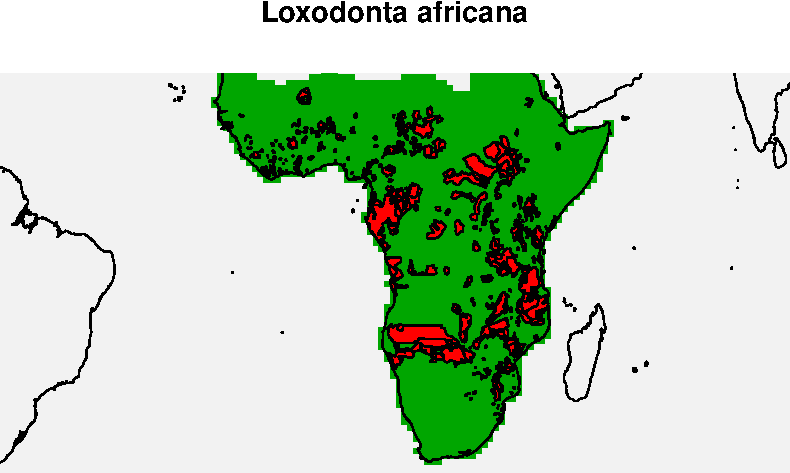
\includegraphics{tutorial_3_files/figure-latex/unnamed-chunk-29-1.pdf}


\end{document}
